\documentclass[oneside]{article}


\author{Philipp Jetzlaff}
\title{Projektdokumentation}

%%%%%%%%%%%%%%%%% P A C K A G E S %%%%%%%%%%%%%%%%%%%%%%%%%%%%%%%%%%%%%%%%%%%%%%%%%%%%%
%Package to create a custom header, that is printed on every page in the document.
\usepackage{fancyhdr}
%Package to include graphics.
\usepackage{graphicx}
%Package to defines the paper enviroment
\usepackage[a4paper, headheight=55pt, bottom=20mm]{geometry}
%Package to defines hyperrefs in the document. E.g references to figures or tables
\usepackage{hyperref}
%Package to use colors in the documents. For example \rowcolor
\usepackage{color, colortbl}
%Define Header
\fancyhf{}
\fancyhead[R]{
\includegraphics[width=0.11\textwidth]{OktoPOS.png}}
\fancyhead[L]{
  \uppercase{Erweiterung eines Onlineserivce}\\
  \vspace{1pt}
  \small{Anbindung der OktoPOS Software an den internen Übersetzungsdienst}\\ 
  \vspace{4pt}
  \scriptsize{\leftmark}
}
\fancyfoot[L]{Philipp Jetzlaff}
\fancyfoot[R]{\thepage}
\renewcommand{\headrulewidth}{1pt}
\renewcommand{\footrulewidth}{1pt}
%Define Colors
\definecolor{LightCyan}{rgb}{0.88,1,1}
\definecolor{blue-green}{rgb}{0.0, 0.87, 0.87}
\definecolor{carolinablue}{rgb}{0.6, 0.73, 0.89}
\definecolor{lightgray}{rgb}{0.83, 0.83, 0.83}
%Define Codeblockfont
%Define imagepath
\graphicspath{{src/img/}}
\renewcommand{\listfigurename}{Abbildungsverzeichnis}
\renewcommand{\contentsname}{Inhaltsverzeichnis}
\renewcommand{\tablename}{Tabelle}
\begin{document}
%Define Header and footer
  \pagestyle{fancy}
  
  %Deckblatt einfügen
  %table of contents
  \pagenumbering{roman}
  \tableofcontents
  \addcontentsline{toc}{section}{\listfigurename}
  \listoffigures
  \addcontentsline{toc}{section}{\listtablename}
  \listoftables
  \newpage
  \section{Verzeichnis der Listings}
  \newpage
  \section{Glossar}
  \newpage
  \pagenumbering{arabic}
  \section{Einleitung}
    Im Rahmen der Abschlussarbeit für den Ausbildungberuft Fachinformatiker für Anwendungsentwicklung 
    wurde diese Projektdokumentation angefertigt. Sie dokumentiert den Ablauf und die Herangehensweise 
    welche zur Lösung, der im Vorfeld von dem zuständigen Ausbilder definierten, Aufgabe beigetragen haben. 
    Der Ausbildungsbetrieb OktoPOS Solutions GmbH ist ein mittelständiges Unternehmen mit Hauptsitz in Hamburg.
  \subsection{Projektbeschreibung}
    Das von der OktoPOS Solutions enwickelte Produkt OkotPOS Cash ist ein, im international Raum, genutztes POS System. 
    Für eine anwenderfreundliche Nutzung ist die gesamte Textausgabe des Front-End in diversen Sprachen konfigurierbar. Zur Realisierung der Textausgabe in 
    den geforderten Sprachen, werden im Quellcode Platzhalter (Tokens) statt konkreter Texte verwendet. 
    Für jede Sprache gibt genau eine Property Datei, in der die Texte der jeweiligen Sprache als Key-Value Paar hinterlegt sind.
    Die Erweiterung und Wartbarkeit dieser Property Dateien sind nach aktuellem Stand optimierungsbedürftig. 
    Es gibt keine Garantie dafür, dass jede Datei die selbe Anzahl an Tokens beinhalten bzw. es gibt keinen direkten Überblick über den Übersetzungsstand der Dateien. 
    In den meisten Fällen werden die Übersetzungen von unternehmensfremden Personal angefertigt, die mit der Struktur solcher Dateien nicht vertraut sind und daher mehr Zeit in Anspruch nehmen als notwendig.\\
    Der unternehmensinternen Übsersetzungsdienst TranslationService, bietet neben den grundlegenden Funktionen zum Importieren/Exportieren von Tokens und Übersetzung auch ein benutzerfreundlichen Userinterface.
  \subsection{Projektziel}
    Ziel des Projektes ist es, durch die Anbindung der Kassensoftware an den unternehmensinternen Translationservice,
    den Prozess der Übersetzung von dem Releaseprozess zu entkoppeln und Versionsupdates der Übersetzungen während des Livebetriebes zu ermöglichen.
    Im Rahmen des Projektes soll die Integrität des Kassencodes erhalten bleiben. Deshalb ist es nötig den Updateprozess in eine weitere Anwendung zu überführen. 
    Die Anforderungen der Anwendung sind aus dem Soll-Konzept zu entnehmen.\\
    Der Transaltionservice ist zu so zu erweitern, dass Tokens und Übersetzungen in Abhängigkeit ihrer Version an den Translationservice gesendet bzw. geladen werden können.
    Nach aktuellem Stand, ist der Translationservice nicht in der Lagen die Tokens und Übersetzungen zu Versionieren. Das Anelgen einer neuen Version erfolgt von außen über eine zu schaffende Schnittstelle.
    Im Front-End des Translationservice, soll die Möglichkeit gegeben werden die Tokens und den Stand der Übersetzung nach ihrer Version anzuzeigen.
    Da das Erstellen der Schnittstellen, die Implementierung der neuen Anwendung, das Testen der Komponenten usw. bereits die veranschlagten 70 Stunden benötigt,
    werden das Deployment der Minianwendung sowie die Anpasssung des Deploymentprozesses der Kassesoftware und die Anpassungen am Frontend als Fremdleistung an eine andere Abteilung weitergegeben. 
  \subsection{Projektumfeld}
    Primär ist das Projekt ein Auftrag der Entwicklungsabteilung des Kassensystems. Das Java gestützte POS System nutzt Übersetzungsdateien um Textstellen im Front-End in verschiedenen Sprachen darzustellen.
    Während der Entwicklung an der Kasse, speziell beim implementieren von Features, werden in machen Fällen neue Übersetzungstokens eingeführt. Der Entwickler muss dabei den Token in jede einzelne Datei schreiben. 
    Die Übersetzer des Tochterunternehmens OktoCareer nutzen den Translationserivce für die Übersetzungen an dem Personalmanagementsystem OktoCareer. 
    Der TranslationSerivce bietet eine Datenstruktur, welche mit geringen Aufwand auf die neuen Anforderungen angepasst werden kann, und die grundlegende Struktur für die RESTFull API. 
  \subsection{Projektabgrenzung}
    Die beschränkte Dauer die für dieses Projekt zur Verfügung gestellt wurde, führt dazu das Teile zur Realisierung des Gesamtprojektes an andere Abteilungen ausgelagert werden müssen.
    Dazu gehören die Anpassungen im Front-End des TransaltionService, sowie das Einrichten des GitWebhooks für die Kassensoftware. Ein bereits vorhandener Service hat bereits die Möglichkeit die Übersetzungsdateien 
    der Kasse in das geplante Format für die Schnittstellen des TranslationService konvertieren. 
  \section{Projektplanung}
  \subsection{Projektphasen}
    Im Vorfeld des Projektes wurden die zu Verfügung stehenden 70 Entwicklerstunden auf verschiende Projektphasen aufgeteilt. Die Zeiteinteilung sowie die einezlene Projektphasen wurden in einer groben Tabelle (\hyperref[tab:timing]{Tabelle 1: Grobe Zeiplanung}) zusammengefasst.
    Eine genaue Zeitplanung inklusive der Aufgaben jeder einzelnen Phase können aus dem \hyperref[sec:detailTime]{Anhang \ref{sec:detailTime}} entnommen werden.
    \begin{table}[h]
      \label{tab:timing}
      \centering
    \begin{tabular}{| l | r |}
      \rowcolor{carolinablue}
      Projektphase & Stunden \\
      \hline
      Analysephase & 7h \\
      \hline
      \rowcolor{lightgray}
      Entwurfsphase & 11h\\
      \hline
      Implementierungsphase & 35h\\
      \hline
      \rowcolor{lightgray}
      Abnahme und Testphase & 3h\\
      \hline
      Dokumentation & 14h \\
      \hline
      \rowcolor{carolinablue}
      Gesamtstunden & 70h
    \end{tabular}
    \caption{Grobe Zeitplanung}
  \end{table}
    Um die zeitliche Abfolge der einzelnen Projektphase grafisch darzustellen, wurden die einzelnen Aufgaben aus den Projektphasen in sinngemäße Aufgaben zusammengefasst und ein Gantt-Chart überführt \hyperref[sec:GanttChart]{Anhang \ref{sec:GanttChart}}.
  \subsection{Vorgehensmodel}
    Zu Beginn des Projektes wurde eine agile Softwareentwicklung in Anlehnung zu
  \subsection{Resourcenplanung}
  \section{Analysephase}
  \subsection{Ist-Analyse}
  \begin{figure}[h]
    \centering
    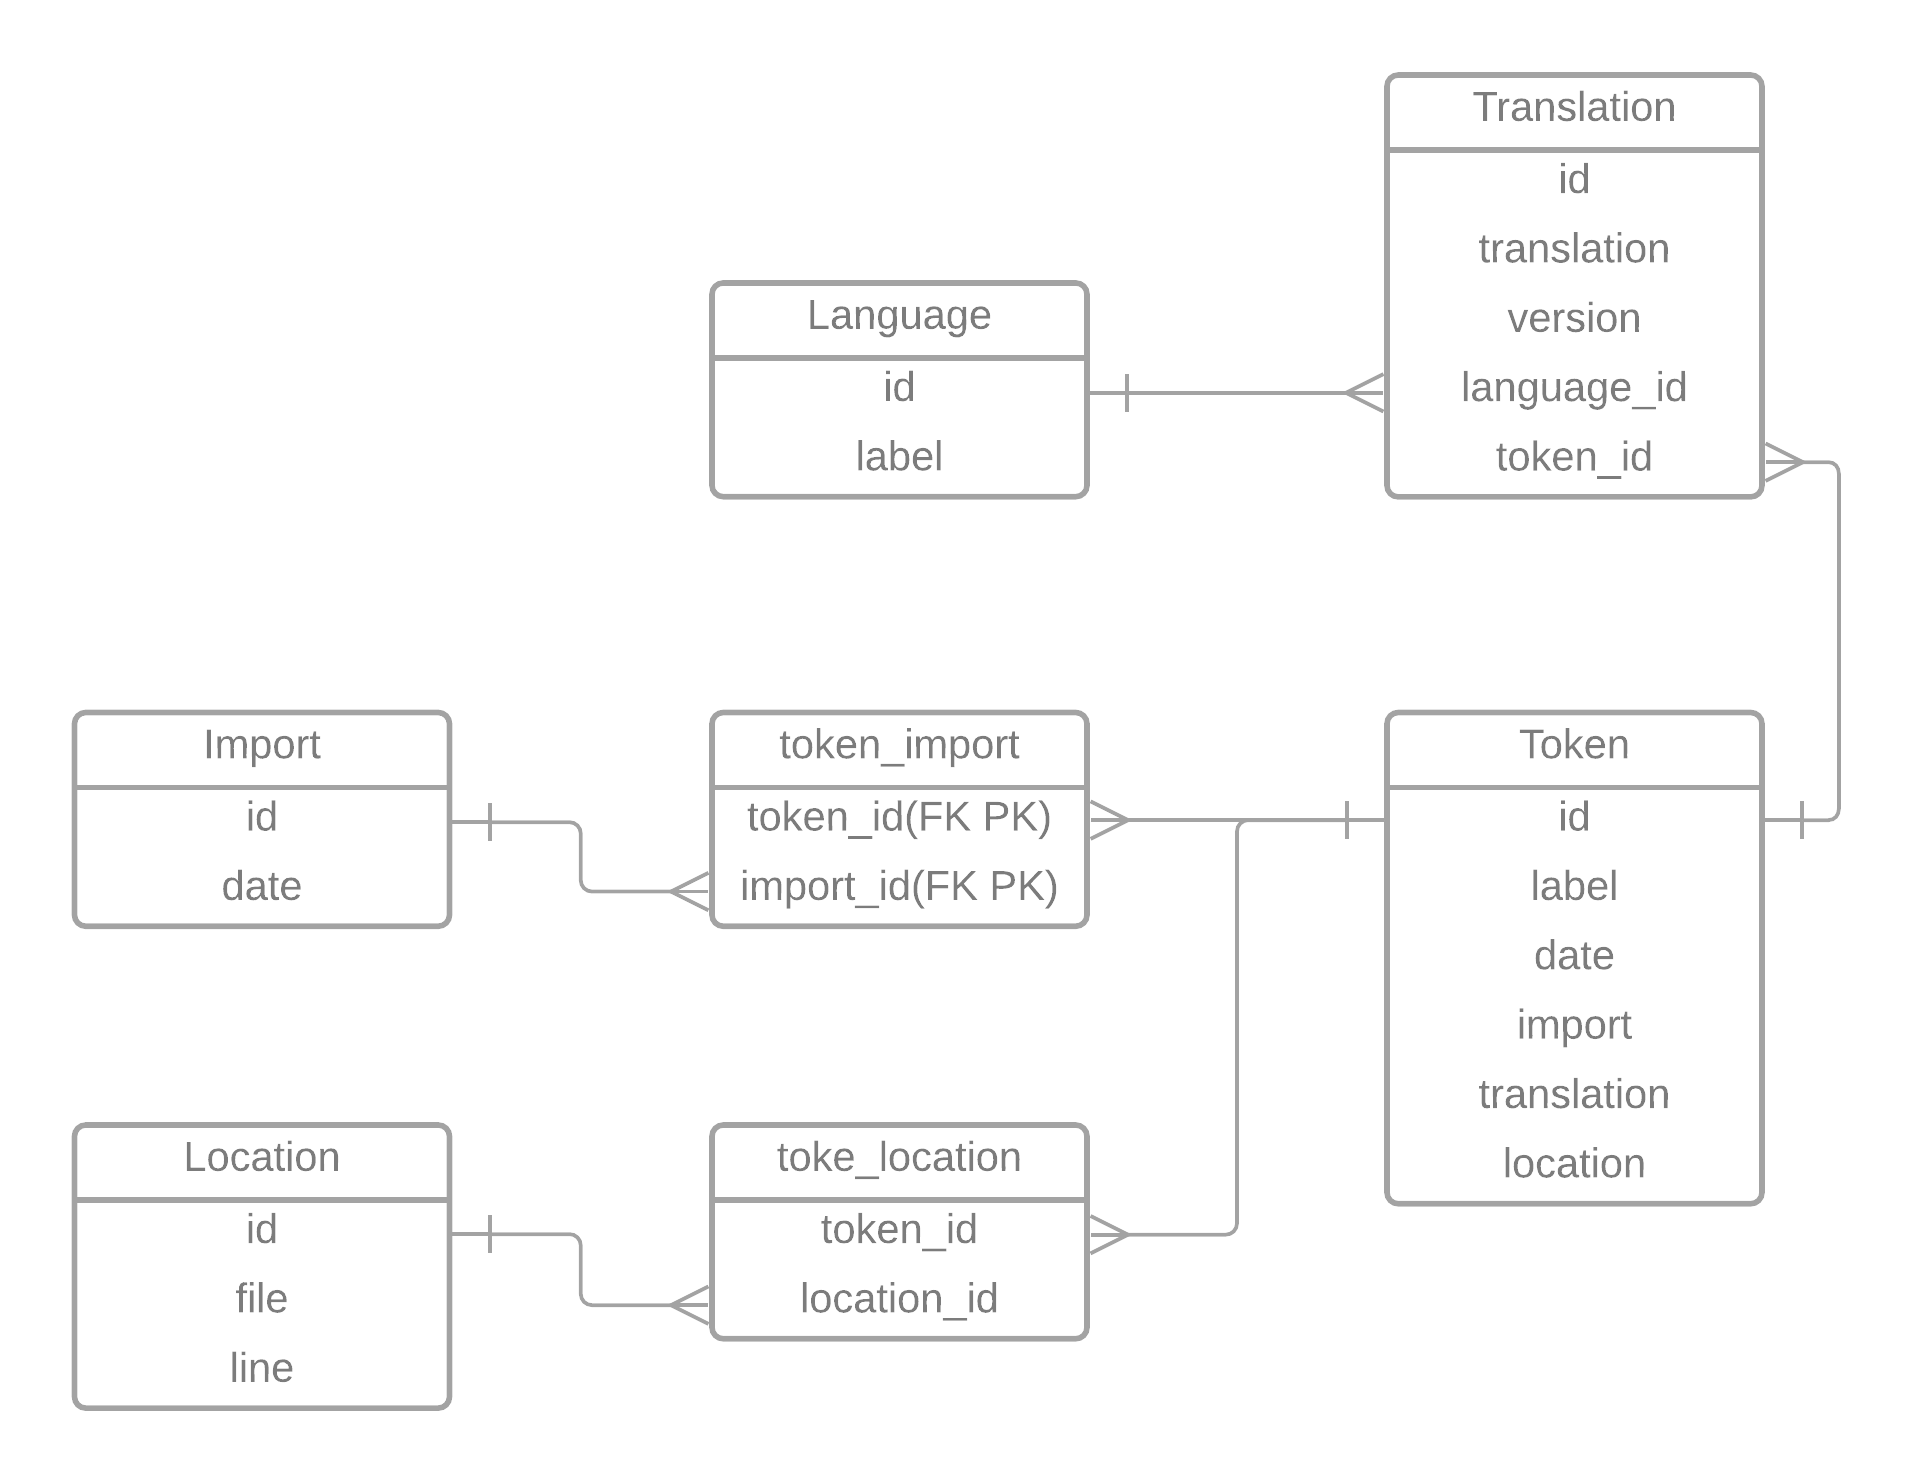
\includegraphics[width=\textwidth]{ERD_TranslationService_IST-Analyse.png}
    \caption{ERD im IST Zustand}
  \end{figure}
  \newpage
  \subsection{Soll-Analyse}
  asd
  \begin{figure}[h]
    \centering
    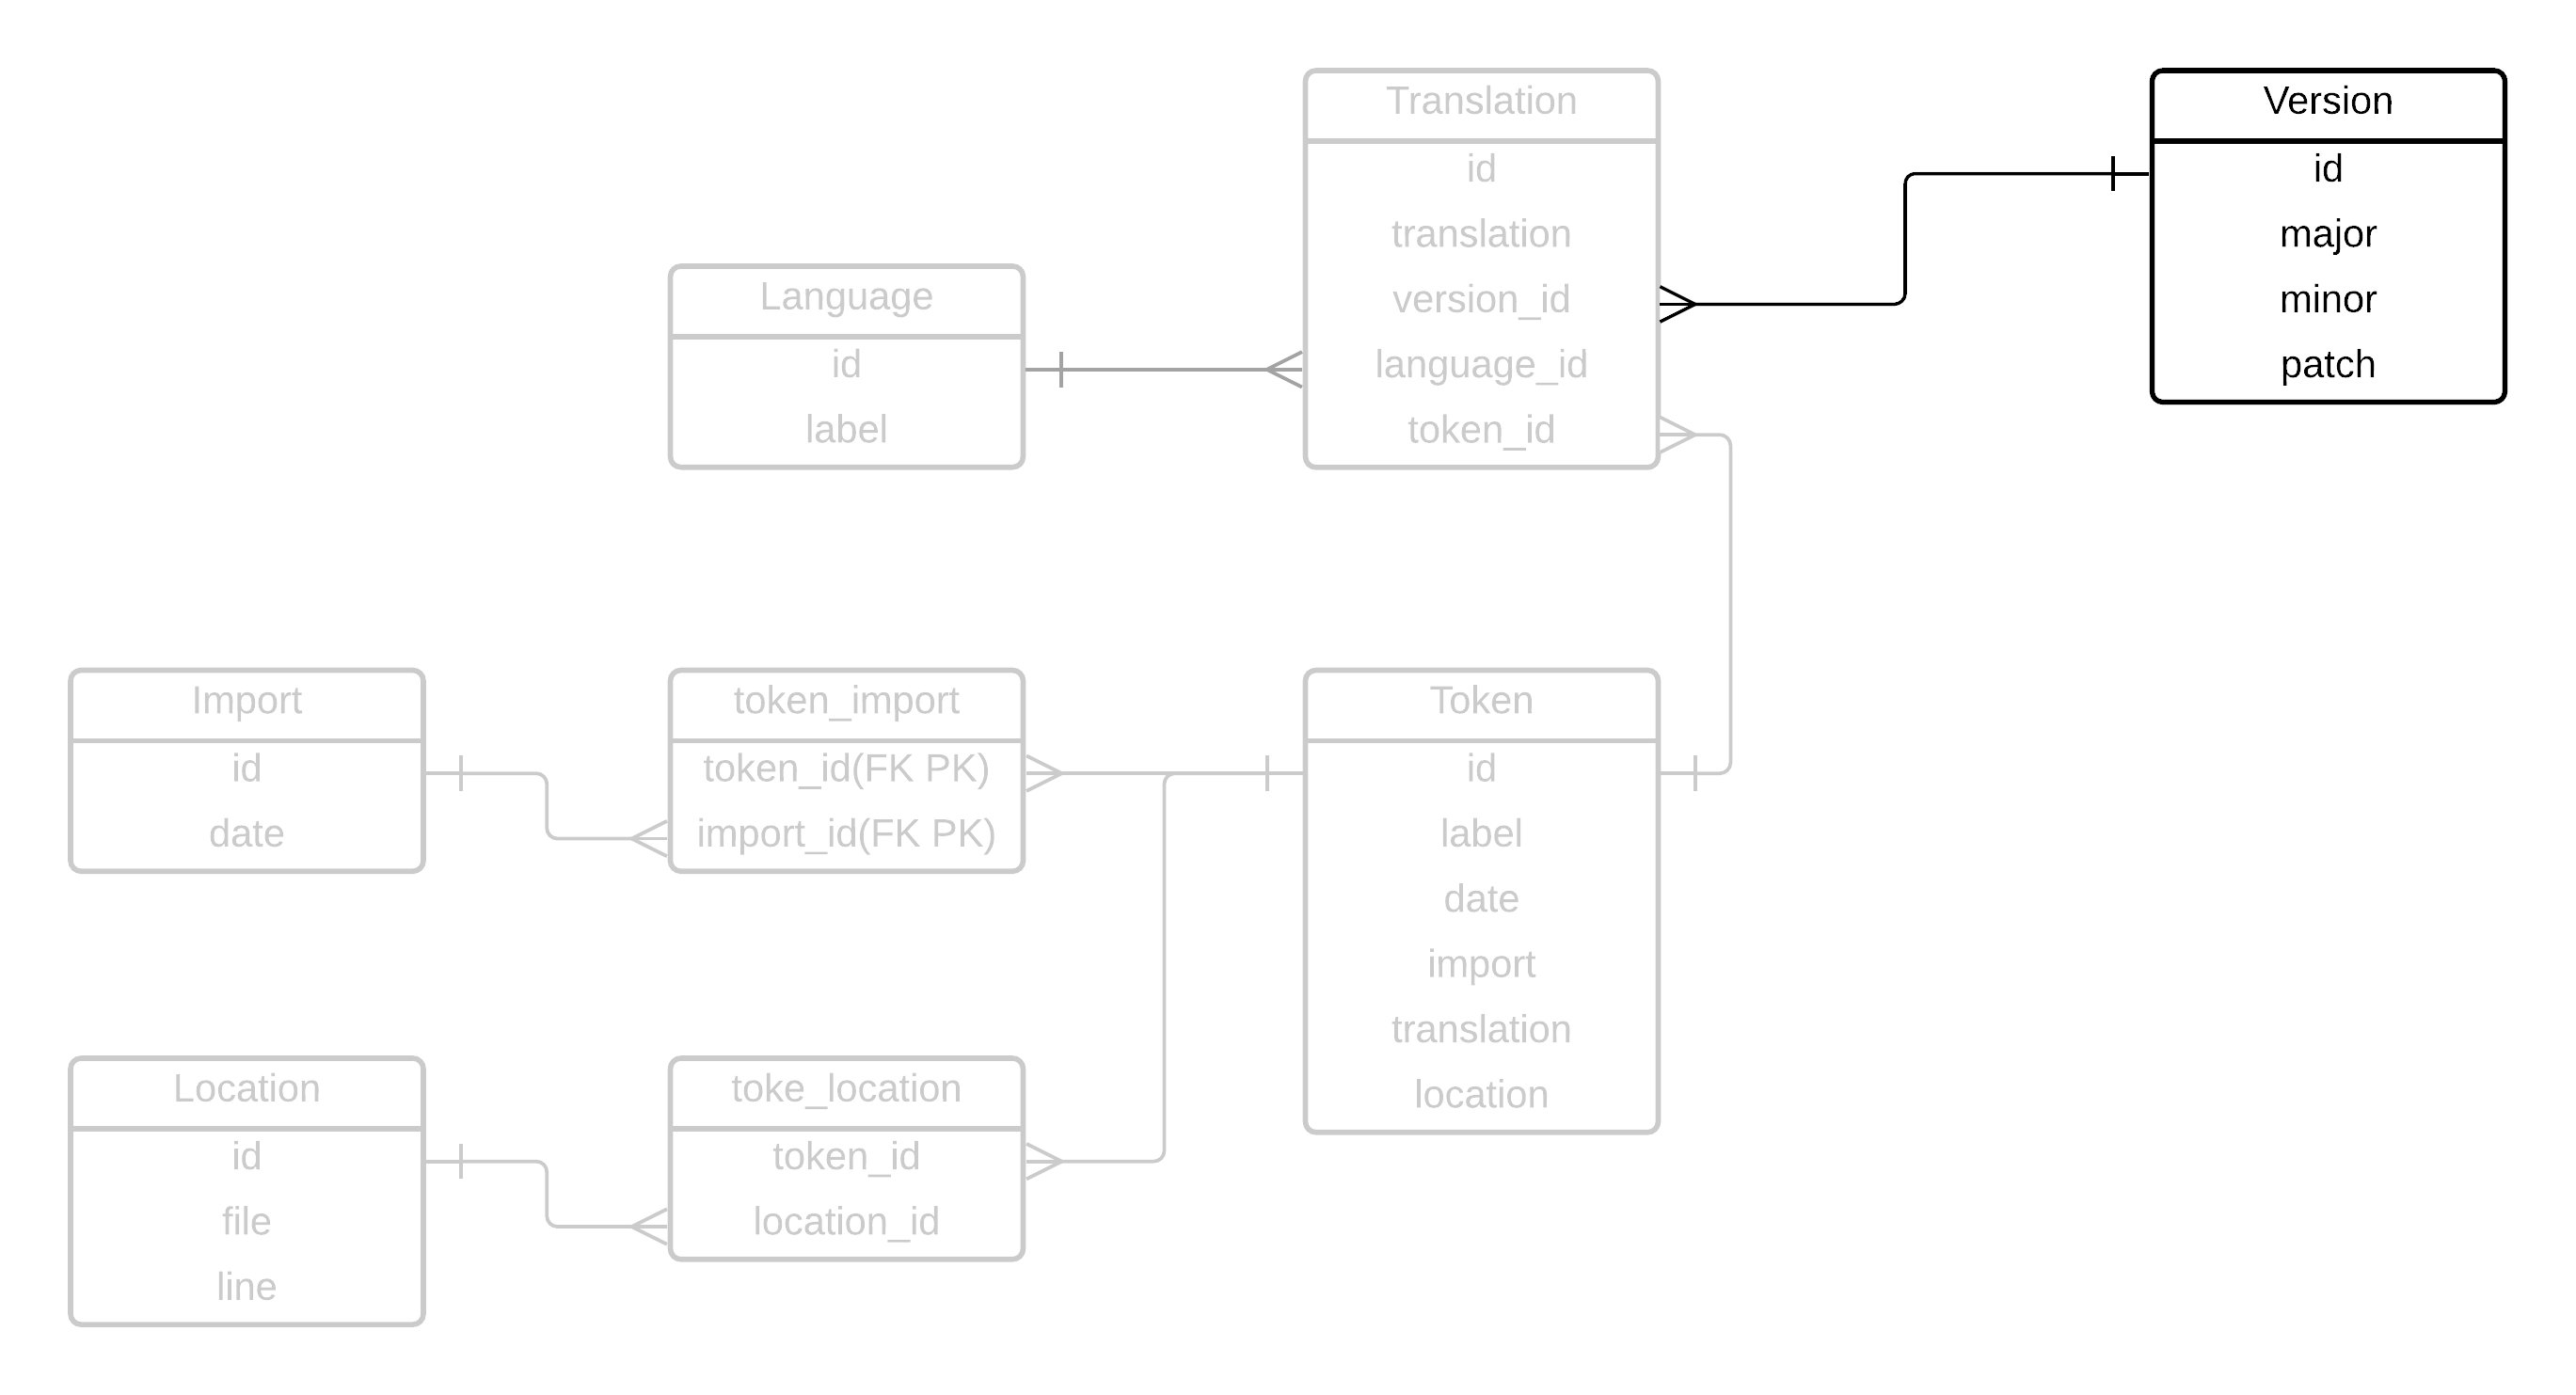
\includegraphics[width=\textwidth]{ERD_TranslationService_SOLL-Analyse.png}
    \caption{ERD im SOLL Zustand}
  \end{figure}  
  \subsection{Wirtschaftsanalyse}
  \subsubsection{Kostenaufstellung}
  \subsubsection{Aromatisierungsdauer}
  \subsection{Anwendungsfälle}
  \subsection{Lastenheft}
  \section{Entwurfsphase}
  \subsection{Userinterface}
  \subsection{Datenmodell}
  \subsection{APIs}
  \subsection{Geschäftslogik}
  \subsection{Testcases}
  \subsection{Pflichtenheft}
  \section{Implementierungsphase}
  \subsection{Translationservice}
  \subsubsection{Erweiterung der bestehenen Datengrundlage}
  \subsubsection{Implemetierung der REST Api}
  \subsection{Translationloader}
  \subsubsection{Geschäftslogik}
  \subsubsection{Userinterface}
  \subsubsection{Batch Script Extension}
  \subsubsection{Webhook}
  \section{Abnahme- und Einführungsphase}
  \subsection{Abnahme durch den Fachbereich}
  \subsection{Deployment}
  \section{Dokumentation}
  \section{Retroanalyse}
  \subsection{IST-SOLL-Vergleich}
  \subsection{Ausblick}
  \setcounter{section}{0}
  \renewcommand{\thesection}{\MakeUppercase{\alph{section}}}
  \section{Anhang}
  \subsection{Detaillierte Zeitplanung}\label{sec:detailTime}
  \subsection{Gantt-Chart}\label{sec:GanttChart}
    Gantt Chart will follow!
    \newpage
  
    
  \subsection{Schnittstelledokumentation}
    \label{interfaceDocumentation}
  Swagger
\end{document}